\documentclass[a4paper]{article}

\usepackage[a4paper,width=150mm,top=25mm,bottom=25mm]{geometry}
\usepackage[utf8x]{inputenc}
\usepackage{amsmath}
\usepackage{graphicx}
\usepackage{subfig}
\usepackage[table]{xcolor}

\title{Homework 3: Report \\ Advanced Data Analysis in Python}
\author{Alper Yıldırım}

\begin{document}
\maketitle

\subsection*{Introduction}
	In this homework assignment, the survey results of CSES Module 4 were examined to apply machine learning algorithms and data analysis. For the analysis, educational level, employment type (Private/Public/Mixed/Non-profit Sector), and socioeconomic status were selected as explanatory variables while the voting behavior (Voted/Not Voted) was target variable. The missing data was imputed using \verb|SimpleImputer| based on the mean of each column. The explanatory variables were scaled through \verb|StandardScaler| which module standardizes variables by removing the mean and scaling to unit variance. For the purpose of model prediction, the data was split as 30\% of test data and 70\% of training data using \verb|train_test_split| module. I applied K-Nearest Neighbors, Gaussian Naive Bayes, and Logistic Regression models to CSES data in order to select best predictive model.

\subsection*{K-Nearest Neighbors Algorithm}

    The accuracy score of K-Nearest Neighbors algorithm is equal to .798 in the model. As Figure 1(a) demonstrates, the best choice of number of neighbors is 5, since low number of neighbors causes higher influence of the noise whereas the high number of neighbors are computationally expensive. Yet, at the cost of computational expensiveness, the number of neighbors can be increased from 5 to 7 to achieve better accuracy scores. Furthermore, Figure 1(b) shows that the rate of True Positives is 77.44\% and of True Negatives is 2.41\%. Inaccuracies in the model mainly caused by False Positive rate of 14.75\% which means that the model predicted some people as 'voted' while they actually do not vote. Lastly, the 10-fold cross validation scores for K-Nearest Neighbors algorithm exhibited in Table 1.
    
\begin{figure}[htbp!]
    \centering
    \subfloat[Number of Neighbors]{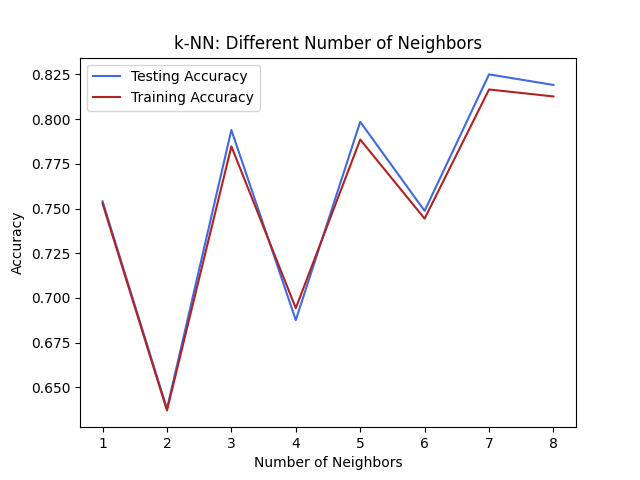
\includegraphics[width=0.5\textwidth]{Visualizations/knn_plot.png}\label{fig:f1}}
    \hfill
    \subfloat[Confusion Matrix]{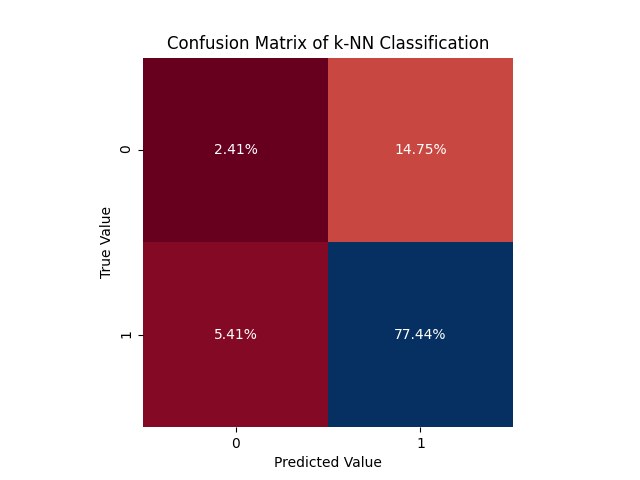
\includegraphics[width=0.5\textwidth]{Visualizations/knn_conf.png}\label{fig:f2}}
    \caption{Results of the k-NN Algorithm}
\end{figure}

\begin{table}[htbp!]
\centering
\begin{tabular}{ |c|c|c|c|c|c|c|c|c|c| } 
 \hline
 \multicolumn{10}{|c|}{\textbf{Cross Validation Scores}} \\
 \hline
 0.8188 & 0.8177 & 0.8130 & 0.7936 & 0.8177 & 0.8186 & 0.8025 & 0.7428 & 0.7738 & 0.7566 \\ 
 \hline
\end{tabular}
\caption{Cross Validation Scores for K-Nearest Neighbors, \textit{k=5}}
\end{table}

\subsection*{Gaussian Naive Bayes Algorithm}

    The accuracy score of Gaussian Naive Bayes algorithm equals to .828. However, as Figure 2 demonstrated, the model predicted all values as positives. Therefore, there is no True Negatives and False Negatives in the model. The 5-fold cross validation scores for Gaussian Naive Bayes algorithm, exhibited in Table 2 below, also imply that bizarre fashion either.

\begin{figure}[htbp!]
    \centering
    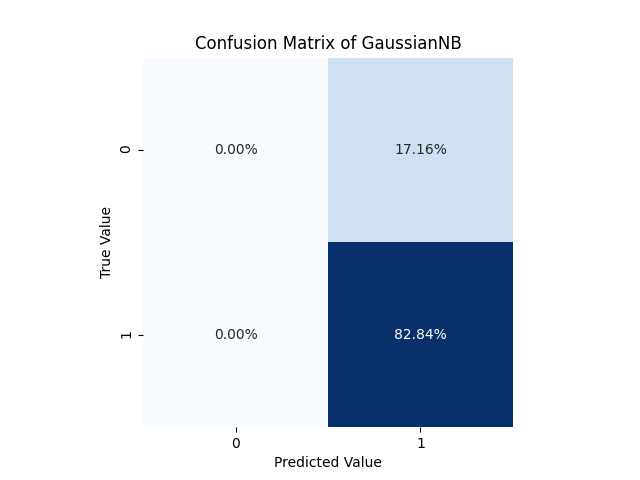
\includegraphics[width=7cm]{Visualizations/gnb_conf.png}
    \caption{Confusion Matrix of Gaussian Naive Bayes}
\end{figure}

\begin{table}[htbp!]
\centering
\begin{tabular}{ |c|c|c|c|c| } 
 \hline
 \multicolumn{5}{|c|}{\textbf{Cross Validation Scores}} \\
 \hline
 0.8187 & \cellcolor[HTML]{B8D8FF}0.8181 & \cellcolor[HTML]{B8D8FF}0.8181 & \cellcolor[HTML]{B8D8FF}0.8181 & \cellcolor[HTML]{B8D8FF}0.8181 \\ 
 \hline
\end{tabular}
\caption{Cross Validation Scores for Gaussian Naive Bayes}
\end{table}

\subsection*{Logistic Regression}

     Logistic Regression algorithm had the accuracy score of .828 which score is exactly same with the accuracy score of Gaussian Naive Bayes algorithm. While the equality of these two scores is odd, this equality is achieved with different combinations of training and test splits either. Moreover, for the purpose of hyper-parameter optimization, different values of regularization strength applied in \verb|GridSearchCV|. The optimal value that model found is equal to .001 which means logistic regression was executed in a highly regularized manner. Lastly, since the model predicted all values Positive, same as Gaussian Naive Bayes once again, Python returned an error in classification report.
    
\begin{figure}[htbp!]
    \centering
    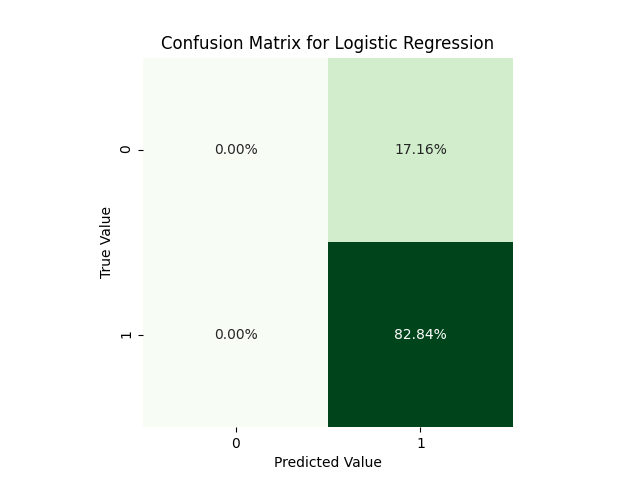
\includegraphics[width=7cm]{Visualizations/logreg_conf.png}
    \caption{Confusion Matrix of Logistic Regression}
\end{figure}

\end{document}
